\chapter{The House at Auteuil}

Monte Cristo noticed, as they descended the staircase, that Bertuccio
signed himself in the Corsican manner; that is, had formed the sign of
the cross in the air with his thumb, and as he seated himself in the
carriage, muttered a short prayer. Anyone but a man of exhaustless
thirst for knowledge would have had pity on seeing the steward’s
extraordinary repugnance for the count’s projected drive without the
walls; but the count was too curious to let Bertuccio off from this
little journey. In twenty minutes they were at Auteuil; the steward’s
emotion had continued to augment as they entered the village.
Bertuccio, crouched in the corner of the carriage, began to examine
with a feverish anxiety every house they passed.

“Tell them to stop at Rue de la Fontaine, No. 28,” said the count,
fixing his eyes on the steward, to whom he gave this order.

Bertuccio’s forehead was covered with perspiration; however, he obeyed,
and, leaning out of the window, he cried to the coachman,—“Rue de la
Fontaine, No. 28.” No. 28 was situated at the extremity of the village;
during the drive night had set in, and darkness gave the surroundings
the artificial appearance of a scene on the stage. The carriage
stopped, the footman sprang off the box and opened the door.

“Well,” said the count, “you do not get out, M. Bertuccio—you are going
to stay in the carriage, then? What are you thinking of this evening?”

Bertuccio sprang out, and offered his shoulder to the count, who, this
time, leaned upon it as he descended the three steps of the carriage.

“Knock,” said the count, “and announce me.”

Bertuccio knocked, the door opened, and the concierge appeared.

“What is it?” asked he.

“It is your new master, my good fellow,” said the footman. And he held
out to the concierge the notary’s order.

“The house is sold, then?” demanded the concierge; “and this gentleman
is coming to live here?”

“Yes, my friend,” returned the count; “and I will endeavor to give you
no cause to regret your old master.”

“Oh, monsieur,” said the concierge, “I shall not have much cause to
regret him, for he came here but seldom; it is five years since he was
here last, and he did well to sell the house, for it did not bring him
in anything at all.”

“What was the name of your old master?” said Monte Cristo.

“The Marquis of Saint-Méran. Ah, I am sure he has not sold the house
for what he gave for it.”

“The Marquis of Saint-Méran!” returned the count. “The name is not
unknown to me; the Marquis of Saint-Méran!” and he appeared to
meditate.

“An old gentleman,” continued the concierge, “a staunch follower of the
Bourbons; he had an only daughter, who married M. de Villefort, who had
been the king’s attorney at Nîmes, and afterwards at Versailles.”

Monte Cristo glanced at Bertuccio, who became whiter than the wall
against which he leaned to prevent himself from falling.

“And is not this daughter dead?” demanded Monte Cristo; “I fancy I have
heard so.”

“Yes, monsieur, one-and-twenty years ago; and since then we have not
seen the poor marquis three times.”

“Thanks, thanks,” said Monte Cristo, judging from the steward’s utter
prostration that he could not stretch the cord further without danger
of breaking it. “Give me a light.”

“Shall I accompany you, monsieur?”

“No, it is unnecessary; Bertuccio will show me a light.”

And Monte Cristo accompanied these words by the gift of two gold
pieces, which produced a torrent of thanks and blessings from the
concierge.

“Ah, monsieur,” said he, after having vainly searched on the
mantle-piece and the shelves, “I have not got any candles.”

“Take one of the carriage-lamps, Bertuccio,” said the count, “and show
me the apartments.”

The steward obeyed in silence, but it was easy to see, from the manner
in which the hand that held the light trembled, how much it cost him to
obey. They went over a tolerably large ground floor; a first floor
consisted of a salon, a bathroom, and two bedrooms; near one of the
bedrooms they came to a winding staircase that led down to the garden.

“Ah, here is a private staircase,” said the count; “that is convenient.
Light me, M. Bertuccio, and go first; we will see where it leads to.”

“Monsieur,” replied Bertuccio, “it leads to the garden.”

“And, pray, how do you know that?”

“It ought to do so, at least.”

“Well, let us be sure of that.”

Bertuccio sighed, and went on first; the stairs did, indeed, lead to
the garden. At the outer door the steward paused.

“Go on, Monsieur Bertuccio,” said the count.

But he who was addressed stood there, stupefied, bewildered, stunned;
his haggard eyes glanced around, as if in search of the traces of some
terrible event, and with his clenched hands he seemed striving to shut
out horrible recollections.

“Well!” insisted the Count.

“No, no,” cried Bertuccio, setting down the lantern at the angle of the
interior wall. “No, monsieur, it is impossible; I can go no farther.”

“What does this mean?” demanded the irresistible voice of Monte Cristo.

“Why, you must see, your excellency,” cried the steward, “that this is
not natural; that, having a house to purchase, you purchase it exactly
at Auteuil, and that, purchasing it at Auteuil, this house should be
No. 28, Rue de la Fontaine. Oh, why did I not tell you all? I am sure
you would not have forced me to come. I hoped your house would have
been some other one than this; as if there was not another house at
Auteuil than that of the assassination!”

“What, what!” cried Monte Cristo, stopping suddenly, “what words do you
utter? Devil of a man, Corsican that you are—always mysteries or
superstitions. Come, take the lantern, and let us visit the garden; you
are not afraid of ghosts with me, I hope?”

Bertuccio raised the lantern, and obeyed. The door, as it opened,
disclosed a gloomy sky, in which the moon strove vainly to struggle
through a sea of clouds that covered her with billows of vapor which
she illumined for an instant, only to sink into obscurity. The steward
wished to turn to the left.

“No, no, monsieur,” said Monte Cristo. “What is the use of following
the alleys? Here is a beautiful lawn; let us go on straight forwards.”

Bertuccio wiped the perspiration from his brow, but obeyed; however, he
continued to take the left hand. Monte Cristo, on the contrary, took
the right hand; arrived near a clump of trees, he stopped. The steward
could not restrain himself.

“Move, monsieur—move away, I entreat you; you are exactly in the spot!”

“What spot?”

“Where he fell.”

\begin{figure}[ht]
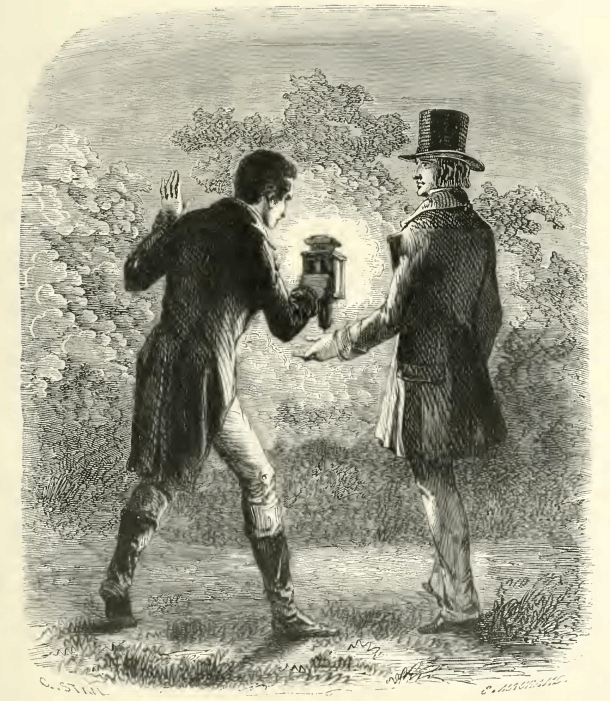
\includegraphics[width=\textwidth]{20281m.jpg}
\end{figure}

“My dear Monsieur Bertuccio,” said Monte Cristo, laughing, “control
yourself; we are not at Sartène or at Corte. This is not a Corsican
\textit{maquis} but an English garden; badly kept, I own, but still you must
not calumniate it for that.”

“Monsieur, I implore you do not stay there!”

“I think you are going mad, Bertuccio,” said the count coldly. “If that
is the case, I warn you, I shall have you put in a lunatic asylum.”

“Alas! excellency,” returned Bertuccio, joining his hands, and shaking
his head in a manner that would have excited the count’s laughter, had
not thoughts of a superior interest occupied him, and rendered him
attentive to the least revelation of this timorous conscience. “Alas!
excellency, the evil has arrived!”

“M. Bertuccio,” said the count, “I am very glad to tell you, that while
you gesticulate, you wring your hands and roll your eyes like a man
possessed by a devil who will not leave him; and I have always
observed, that the devil most obstinate to be expelled is a secret. I
knew you were a Corsican. I knew you were gloomy, and always brooding
over some old history of the vendetta; and I overlooked that in Italy,
because in Italy those things are thought nothing of. But in France
they are considered in very bad taste; there are gendarmes who occupy
themselves with such affairs, judges who condemn, and scaffolds which
avenge.”

Bertuccio clasped his hands, and as, in all these evolutions, he did
not let fall the lantern, the light showed his pale and altered
countenance. Monte Cristo examined him with the same look that, at
Rome, he had bent upon the execution of Andrea, and then, in a tone
that made a shudder pass through the veins of the poor steward—

“The Abbé Busoni, then told me an untruth,” said he, “when, after his
journey in France, in 1829, he sent you to me, with a letter of
recommendation, in which he enumerated all your valuable qualities.
Well, I shall write to the abbé; I shall hold him responsible for his
\textit{protégé’s} misconduct, and I shall soon know all about this
assassination. Only I warn you, that when I reside in a country, I
conform to all its code, and I have no wish to put myself within the
compass of the French laws for your sake.”

“Oh, do not do that, excellency; I have always served you faithfully,”
cried Bertuccio, in despair. “I have always been an honest man, and, as
far as lay in my power, I have done good.”

“I do not deny it,” returned the count; “but why are you thus agitated.
It is a bad sign; a quiet conscience does not occasion such paleness in
the cheeks, and such fever in the hands of a man.”

“But, your excellency,” replied Bertuccio hesitatingly, “did not the
Abbé Busoni, who heard my confession in the prison at Nîmes, tell you
that I had a heavy burden upon my conscience?”

“Yes; but as he said you would make an excellent steward, I concluded
you had stolen—that was all.”

“Oh, your excellency!” returned Bertuccio in deep contempt.

“Or, as you are a Corsican, that you had been unable to resist the
desire of making a ‘stiff,’ as you call it.”

“Yes, my good master,” cried Bertuccio, casting himself at the count’s
feet, “it was simply vengeance—nothing else.”

“I understand that, but I do not understand what it is that galvanizes
you in this manner.”

“But, monsieur, it is very natural,” returned Bertuccio, “since it was
in this house that my vengeance was accomplished.”

“What! my house?”

“Oh, your excellency, it was not yours, then.”

“Whose, then? The Marquis de Saint-Méran, I think, the concierge said.
What had you to revenge on the Marquis de Saint-Méran?”

“Oh, it was not on him, monsieur; it was on another.”

“This is strange,” returned Monte Cristo, seeming to yield to his
reflections, “that you should find yourself without any preparation in
a house where the event happened that causes you so much remorse.”

“Monsieur,” said the steward, “it is fatality, I am sure. First, you
purchase a house at Auteuil—this house is the one where I have
committed an assassination; you descend to the garden by the same
staircase by which he descended; you stop at the spot where he received
the blow; and two paces farther is the grave in which he had just
buried his child. This is not chance, for chance, in this case, is too
much like Providence.”

“Well, amiable Corsican, let us suppose it is Providence. I always
suppose anything people please, and, besides, you must concede
something to diseased minds. Come, collect yourself, and tell me all.”

“I have related it but once, and that was to the Abbé Busoni. Such
things,” continued Bertuccio, shaking his head, “are only related under
the seal of confession.”

“Then,” said the count, “I refer you to your confessor. Turn Chartreux
or Trappist, and relate your secrets, but, as for me, I do not like
anyone who is alarmed by such phantasms, and I do not choose that my
servants should be afraid to walk in the garden of an evening. I
confess I am not very desirous of a visit from the commissary of
police, for, in Italy, justice is only paid when silent—in France she
is paid only when she speaks. \textit{Peste!} I thought you somewhat Corsican,
a great deal smuggler, and an excellent steward; but I see you have
other strings to your bow. You are no longer in my service, Monsieur
Bertuccio.”

“Oh, your excellency, your excellency!” cried the steward, struck with
terror at this threat, “if that is the only reason I cannot remain in
your service, I will tell all, for if I quit you, it will only be to go
to the scaffold.”

“That is different,” replied Monte Cristo; “but if you intend to tell
an untruth, reflect it were better not to speak at all.”

“No, monsieur, I swear to you, by my hopes of salvation, I will tell
you all, for the Abbé Busoni himself only knew a part of my secret;
but, I pray you, go away from that plane-tree. The moon is just
bursting through the clouds, and there, standing where you do, and
wrapped in that cloak that conceals your figure, you remind me of M. de
Villefort.”

“What!” cried Monte Cristo, “it was M. de Villefort?”

“Your excellency knows him?”

“The former royal attorney at Nîmes?”

“Yes.”

“Who married the Marquis of Saint-Méran’s daughter?”

“Yes.”

“Who enjoyed the reputation of being the most severe, the most upright,
the most rigid magistrate on the bench?”

“Well, monsieur,” said Bertuccio, “this man with this spotless
reputation——”

“Well?”

“Was a villain.”

“Bah,” replied Monte Cristo, “impossible!”

“It is as I tell you.”

“Ah, really,” said Monte Cristo. “Have you proof of this?”

“I had it.”

“And you have lost it; how stupid!”

“Yes; but by careful search it might be recovered.”

“Really,” returned the count, “relate it to me, for it begins to
interest me.”

And the count, humming an air from \textit{Lucia}, went to sit down on a
bench, while Bertuccio followed him, collecting his thoughts. Bertuccio
remained standing before him.

\begin{figure}[h]
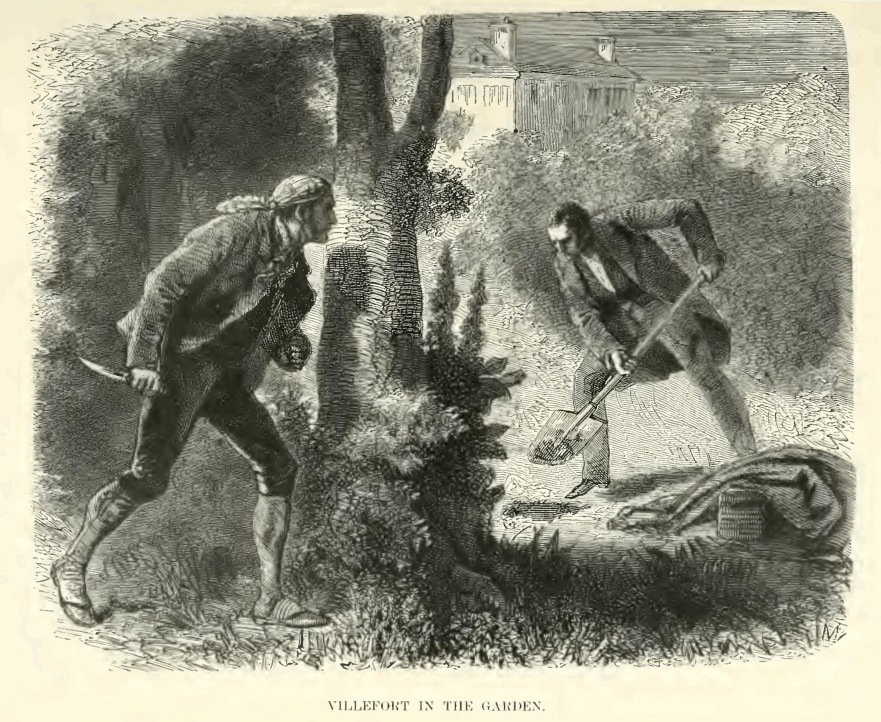
\includegraphics[width=\textwidth]{20285m.jpg}
\end{figure}
